\section{Auditing public releases}
\label{sec:audit}

We ran AugLeak on the official or customary splits of six public image collections and inspected the highest-ranked candidate pairs by eye. Figure~\ref{fig:audit} shows examples and Appendix Table~\ref{tab:audit} summarises the counts. All inspected pairs and our judgements are released.

\begin{figure}[t]
  \centering
  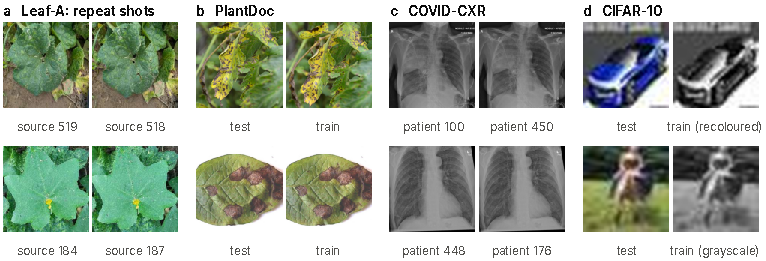
\includegraphics[width=\linewidth]{figs/fig_audit.pdf}
  \caption{\textbf{Examples from the audit}, all confirmed by inspection. (a) Two ``independent'' source photographs that show the same leaf. (b) PlantDoc test images also in training (lower pair: late blight in test, early blight in training). (c) One radiograph filed under two patient identifiers. (d) CIFAR-10 test images whose recoloured or grayscale copy is in the training set.}
  \label{fig:audit}
\end{figure}

\paragraph{Repeat shots defeat file-name groups.}
In both leaf releases, distinct source photographs are often the same physical leaf photographed again moments later. Among the $60$ highest-ranked cross-source pairs of canonical copies, we judged \numRepAyes{} (Leaf-A) and \numRepByes{} (Leaf-B) to show the same leaf; AugLeak links \numRepAlinked{} of Leaf-A's $600$ and \numRepBlinked{} of Leaf-B's $850$ sources to another source at $\alpha=10^{-2}$. A split by file-name group is therefore itself leaky. In each release one source photograph also appears under two classes (Table~\ref{tab:audit}).

\paragraph{PlantDoc.}
Eight of the $236$ official test images~\citep{singh2020plantdoc} ($3.4\%$) are byte-identical to a training image \emph{with a different label} (e.g.\ ``corn gray leaf spot'' in training, ``corn leaf blight'' in test). Among the $40$ top-ranked same-class pairs, \numPDyes{} more test photographs ($5.5\%$) also appear in training, often re-cropped or re-watermarked: at least \numPDtotal{} of the test set is compromised. A linear probe scores \numPDaccDup{} on these and \numPDaccRest{} on the rest.

\paragraph{COVID-19 radiographs.}
In COVID-CXR~\citep{cohen2020covid}, $62.5\%$ of frontal radiographs share a patient with another image, and an image-level split overstates patient-level accuracy by \numCovidLpGap{} (linear probe) and \numCovidKnnGap{} points (1-NN). Patient identifiers are not complete groups either: the top-ranked cross-patient pairs include three radiographs filed under two patient identifiers.

\paragraph{Brain MRI.}
In the official split of a widely used brain-tumour MRI collection~\citep{bhuvaji2020brain}, \numBTexact{} of the \numBTntest{} test images (\numBTexactPct{}), all labelled ``no tumour'', are byte-identical to training images. Hubness correction buried three quarters of them, hence AugLeak's exact-copy rule (Section~\ref{sec:method}). In all it flags \numBTflag{} test images (\numBTflagPct{}) at $\alpha=10^{-2}$, against \numBTcross{} linked to another class, where no copy should exist; all \numBTyes{} top-ranked non-identical pairs we inspected show the same slice. A linear probe scores \numBTaccFlag{} on flagged images and \numBTaccClean{} on the rest: the official \numBTaccAll{} is largely a score on seen slices.

\paragraph{Fruits-360.}
In the official split of Fruits-360~\citep{muresan2018fruits} (15 classes), AugLeak flags \numFRflag{} of \numFRntest{} test images (\numFRflagPct{}) at $\alpha=10^{-3}$. Every flagged pair joins two frames with the same file-name prefix, that is, the same capture sequence of one rotating fruit, a median of six frames apart; all \numFRyes{} pairs we inspected show the same fruit in nearly the same pose. Here the leak does not change the score: a linear probe exceeds $99.9\%$ on flagged and unflagged images alike, because the task is saturated.

\paragraph{CIFAR-10.}
\numCifarText{}
